\documentclass{standalone}
\usepackage{pgfplots}
\usepgfplotslibrary{polar}
\pgfplotsset{compat=1.18}

\begin{document}
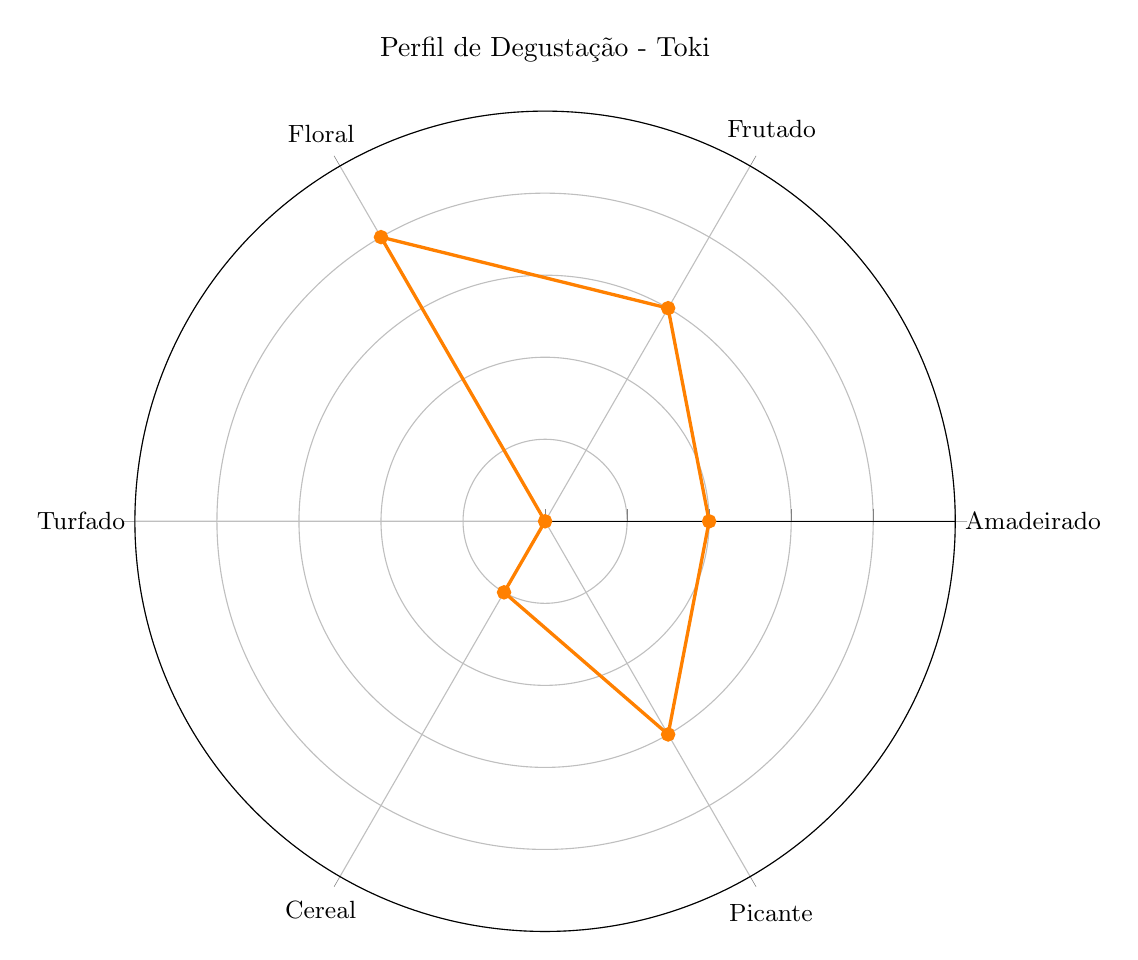
\begin{tikzpicture}
\begin{polaraxis}[
    title={Perfil de Degustação - Toki},
    xtick={0,60,120,180,240,300},
    xticklabels={Amadeirado, Frutado, Floral, Turfado, Cereal, Picante},
    ymin=0, ymax=5,
    ytick={0,1,2,3,4,5},
    yticklabels={,,,},
    xticklabel style={font=\small},
    grid={major},
    width=12cm,
    height=12cm
]
\addplot+[mark=*,mark size=2,very thick,orange,mark options={fill=orange, draw=orange}] coordinates {
    (0,2) %Amadeirado
    (60,3) %Frutado
    (120,4) %Floral
    (180,0) %Turfado
    (240,1) %Cereal
    (300,3) %Picante
} --cycle;
\end{polaraxis}
\end{tikzpicture}
\end{document}
